\documentclass[../main.tex]{subfiles}
\usepackage{chngcntr}

\begin{document}

\chapter{Modeling, Numerical Methods, and Problem Solving}
\pagenumbering{arabic}
\label{cha:cha3}


\begin{center}
\Large{\textbf{CHAPTER OBJECTIVES}}
\end{center}

\normalsize{The primary objective of this chapter is to provide you with a concrete idea of what
numerical methods are and how they relate to engineering and scientific problem
solving. Specific objectives and topics covered are}

\begin{itemize}

\item Learning how mathematical models can be formulated on the basis of scientific

principles to simulate the behavior of a simple physical system.
\item Understanding how numerical methods afford a means to generate solutions in a
manner that can be implemented on a digital computer.

\item Understanding the different types of conservation laws that lie beneath the models
used in the various engineering disciplines and appreciating the difference
between steady-state and dynamic solutions of these models.

\item Learning about the different types of numerical methods we will cover in this
book.

\end{itemize}
\Large{YOU'VE GOT A PROBLEM}


\normalsize{Suppose that a bungee-jumping company hires you. You’re given the task of predicting the velocity of a jumper (Fig. 1.1)  as a function of time during the free-fall part
of the jump. This information will be used as part of a larger analysis to determine the
length and required strength of the bungee cord for jumpers of different mass.
You know from your studies of physics that the acceleration should be equal to the ratio
of the force to the mass (Newton’s second law). Based on this insight and your knowledge of physics and fluid mechanics, you develop the following mathematical model for the rate
of change of velocity with respect to time, }
\newpage


    
\begin{wrapfigure}{l}{0.25\textwidth}
    \centering
    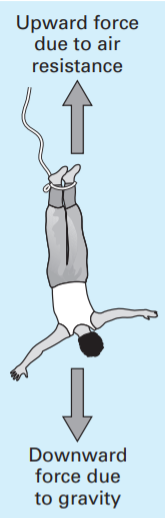
\includegraphics[width=0.25\textwidth]{fig_1_1}
   \caption{\textsf{Forces acting on a free-falling bungee jumper}}
   \label{fig:fig_1_1}
\end{wrapfigure}



$\dfrac{dv}{dt}=g-\dfrac{c_d}{m}v^2$
where $v =$ downward vertical velocity (m/s), $t =$ time (s), $g =$ the acceleration due to
gravity ($\cong$ 9.81 m/s2), $c_d = a$ lumped drag coefficient (kg/m), and $m =$ the jumper’s
mass (kg). The drag coefficient is called “lumped” because its magnitude depends on factors such as the jumper’s area and the fluid density (see Sec 1.4).


Because this is a differential equation, you know that calculus might be used to obtain
an analytical or exact solution for $v$ as a function of $t$. However, in the following pages, we
will illustrate an alternative solution approach. This will involve developing a computeroriented numerical or approximate solution.


Aside from showing you how the computer can be used to solve this particular problem, our more general objective will be to illustrate (a) what numerical methods are and
(b) how they figure in engineering and scientific problem solving. In so doing, we will also
show how mathematical models figure prominently in the way engineers and scientists use
numerical methods in their work.


\bigskip
\section{A SIMPLE MATHEMATICAL MODEL}
\label{sec:sec1}
  A \textsl{mathematical model} can be broadly defined as a formulation or equation that expresses
the essential features of a physical system or process in mathematical terms. In a very general sense, it can be represented as a functional relationship of the form


\begin{equation}
\tag{1.1}
\overset{Dependent}{variable} = f \left( \overset{independent}{variables},parameters,\overset{forcing}{functions}\right)  
\end{equation}
 
where the \textsl{dependent variable} is a characteristic that typically reflects the behavior or state
of the system; the independent variables are usually dimensions, such as time and space,
along which the system’s behavior is being determined; the parameters are reflective of the
system's properties or composition; and the forcing functions are external influences acting
upon it.

The actual mathematical expression of Eq. (1.1) can range from a simple algebraic
relationship to large complicated sets of differential equations. For example, on the basis of
his observations, Newton formulated his second law of motion, which states that the time
rate of change of momentum of a body is equal to the resultant force acting on it. The mathematical expression, or model, of the second law is the well-known equation

\begin{equation}
\tag{1.2}
F=ma
\end{equation}

where $F$ is the net force acting on the body $(N, or kg m/s^2
), m$ is the mass of the object (kg),
and a is its acceleration $(m/s^2
)$.

The second law can be recast in the format of Eq. (1.1) by merely dividing both sides
by $m$ to give
\begin{equation}
\tag{1.3}
a=\dfrac{F}{m}
\end{equation}

where $a$ is the dependent variable reflecting the system's behavior, $F$ is the forcing function, and $m$ is a parameter. Note that for this simple case there is no independent variable
because we are not yet predicting how acceleration varies in time or space.

\begin{itemize}
\item  It describes a natural process or system in mathematical terms.
\item It represents an idealization and simplification of reality. That is, the model ignores negligible details of the natural process and focuses on its essential manifestations. Thus,
the second law does not include the effects of relativity that are of minimal importance
when applied to objects and forces that interact on or about the earth’s surface at velocities and on scales visible to humans.
\item  Finally, it yields reproducible results and, consequently, can be used for predictive purposes. For example, if the force on an object and its mass are known, Eq. (1.3) can be
used to compute acceleration.

\end{itemize}


Because of its simple algebraic form, the solution of Eq. (1.2) was obtained easily.
However, other mathematical models of physical phenomena may be much more complex,
and either cannot be solved exactly or require more sophisticated mathematical techniques
than simple algebra for their solution. To illustrate a more complex model of this kind,
Newton’s second law can be used to determine the terminal velocity of a free-falling body
near the earth’s surface. Our falling body will be a bungee jumper (Fig. 1.1). For this case,
a model can be derived by expressing the acceleration as the time rate of change of the
velocity $(dv/dt)$ and substituting it into Eq. (1.3) to yield

\begin{equation}
\tag{1.4}
\dfrac{dv}{dt}=\dfrac{F}{m}
\end{equation}
where $v$ is velocity (in meters per second). Thus, the rate of change of the velocity is equal
to the net force acting on the body normalized to its mass. If the net force is positive, the
object will accelerate. If it is negative, the object will decelerate. If the net force is zero, the
object's velocity will remain at a constant level.


Next, we will express the net force in terms of measurable variables and parameters.
For a body falling within the vicinity of the earth, the net force is composed of two opposing forces: the downward pull of gravity $F_D$ and the upward force of air resistance $F_U$
(Fig. 1.1):

\begin{equation}
\tag{1.5}
F= F_D + F_U
\end{equation}

If force in the downward direction is assigned a positive sign, the second law can be
used to formulate the force due to gravity as

\begin{equation}
\tag{1.6}
F_D=mg
\end{equation}
where g is the acceleration due to gravity $(9.81 m/s^2
)$.

Air resistance can be formulated in a variety of ways. Knowledge from the science of
fluid mechanics suggests that a good first approximation would be to assume that it is proportional to the square of the velocity,

\begin{equation}
\tag{1.7}
F_U=-c_dv^2
\end{equation}

where $c_d$ is a proportionality constant called the \textsl{lumped drag coefficient} (kg/m). Thus, the
greater the fall velocity, the greater the upward force due to air resistance. The parameter
$c_d$ accounts for properties of the falling object, such as shape or surface roughness, that affect air resistance. For the present case, $c_d$ might be a function of the type of clothing or the
orientation used by the jumper during free fall.
The net force is the difference between the downward and upward force. Therefore,
Eqs. (1.4) through (1.7) can be combined to yield
\begin{equation}
\tag{1.8}
\dfrac{dv}{dt}=g-\dfrac{C_d}{m}v^2
\end{equation}

Equation (1.8) is a model that relates the acceleration of a falling object to the forces
acting on it. It is a \textsl{differential equation} because it is written in terms of the differential rate
of change $(dv/dt)$ of the variable that we are interested in predicting. However, in contrast
to the solution of Newton's second law in Eq. (1.3), the exact solution of Eq. (1.8) for the
velocity of the jumper cannot be obtained using simple algebraic manipulation. Rather,
more advanced techniques such as those of calculus must be applied to obtain an exact or
analytical solution. For example, if the jumper is initially at rest $(v = 0 at t = 0)$, calculus
can be used to solve Eq. (1.8) for

\begin{equation}
\tag{1.9}
v(t)=\sqrt{\dfrac{gm}{c_d}}tanh \left(\sqrt{\dfrac{gc_d}{m}t}\right)
\end{equation}
where tanh is the hyperbolic tangent that can be either computed directly\footnote{{}MATLAB allows direct calculation of the hyperbolic tangent via the built-in function $tanh(x)$.} or via the more
elementary exponential function as in

\begin{equation}
\tag{1.10}
tanhx=\dfrac{e^x-e^{-x}}{e^x+e^{-x}}
\end{equation}

Note that Eq. (1.9) is cast in the general form of Eq. (1.1) where $v(t)$ is the dependent
variable, $t$ is the independent variable, $c_d$ and $m$ are parameters, and $g$ is the forcing function.


\bigskip
\section*{EXAMPLE 1.1. Analytical Solution to the Bungee Jumper Problem }
\label{sec:sec3}
\textbf{Problem Statement.} A bungee jumper with a mass of 68.1 kg leaps from a stationary hot
air balloon. Use Eq. (1.9) to compute velocity for the first 12 s of free fall. Also determine
the terminal velocity that will be attained for an infinitely long cord (or alternatively, the
jumpmaster is having a particularly bad day!). Use a drag coefficient of 0.25 kg/m.

\textbf{Solution.} Inserting the parameters into Eq. (1.9) yields

$$ 
v(t) =\sqrt{\dfrac{9.81(68.1)}{0.25}}tanh \left(\sqrt{\dfrac{9.81(0.25)}{68.1}}t\right)= 51.6938 tanh(0.18977t)
$$
\newpage
which can be used to compute

\begin{figure}[H]
	\centering
	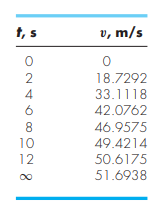
\includegraphics[width=0.25\textwidth]{fig_1_1s}
   \label{fig:fig_1_1s}
\end{figure}



According to the model, the jumper accelerates rapidly (Fig. 1.2). A velocity of
49.4214 m/s (about 110 mi/hr) is attained after 10 s. Note also that after a sufficiently long

\begin{figure}[H]
	\centering
	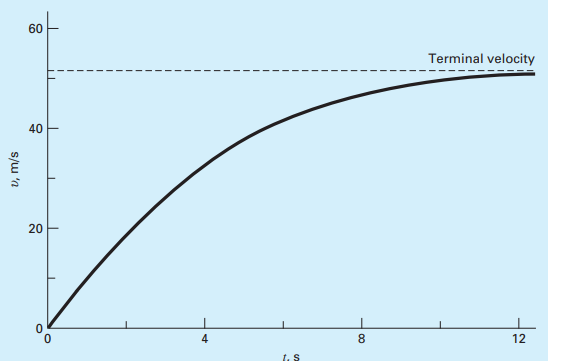
\includegraphics[width=0.75\textwidth]{fig_1_2}
   \caption{\textsf{The analytical solution for the bungee jumper problem as computed in Example 1.1. Velocity
increases with time and asymptotically approaches a terminal velocity.}}
   \label{fig:fig_1_2}
\end{figure}

time, a constant velocity, called the terminal velocity, of 51.6983 m/s (115.6 mi/hr) is
reached. This velocity is constant because, eventually, the force of gravity will be in balance with the air resistance. Thus, the net force is zero and acceleration has ceased.


Equation (1.9) is called an analytical or closed-form solution because it exactly satisfies the original differential equation. Unfortunately, there are many mathematical models
that cannot be solved exactly. In many of these cases, the only alternative is to develop a
numerical solution that approximates the exact solution.
\textit{Numerical methods} are those in which the mathematical problem is reformulated so it
can be solved by arithmetic operations. This can be illustrated for Eq. (1.8) by realizing that
the time rate of change of velocity can be approximated by (Fig. 1.3):

\begin{equation}
\tag{1.11}
\dfrac{dv}{dt}\cong\dfrac{\Delta v}{\Delta t} = \dfrac{v(t_{i+1})-v(t_i)}{t_{i+1}-t_i}
\end{equation}

where $\Delta v$ and $\Delta t$ are differences in velocity and time computed over finite intervals, $v(t_i)$
is velocity at an initial time $t_i$, and $v(t_{i+1})$ is velocity at some later time $(t_{i+1})$. Note that
$dv/dt \cong \Delta v / \Delta t$ is approximate because $ \Delta t$ is finite. Remember from calculus that
$$
\dfrac{dv}{dt} = \lim_{\Delta t\to 0} \dfrac{\Delta v}{ \Delta t}
$$

Equation (1.11) represents the reverse process.

\begin{figure}[H]
	\centering
	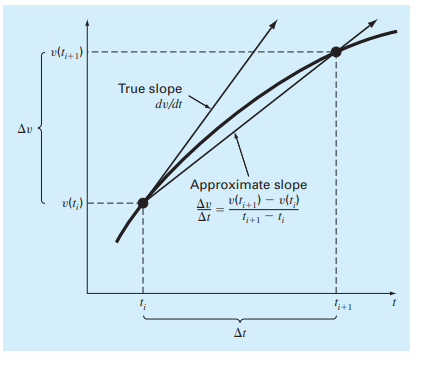
\includegraphics[width=0.75\textwidth]{fig_1_3}
   \caption{\textsf{The use of a finite difference to approximate the first derivative of v with respect to t.}}
   \label{fig:fig_1_3}
\end{figure}

\begin{lstlisting}[numbers=none]
	>> whos
		Name			Size			Bytes			Class
		A			3x3 			72 				double array
		a			1x5 			40 				double array
		ans			1x1 			8 				double array
		b			5x1 			40 				double array
		x			1x1 			16 				double array (complex)
		Grand total is 21 elements using 176 bytes
\end{lstlisting}


\end{document}